\documentclass[10pt]{article}
\usepackage[utf8]{inputenc}
\usepackage[T1]{fontenc}
\usepackage{colormgr}
\usepackage{times}
\usepackage{latexsym}
\usepackage{url}
\usepackage{graphicx}
\usepackage{amsmath}
\usepackage{amssymb}
\usepackage{booktabs}
\usepackage{multirow}
\usepackage{xcolor}
\usepackage{microtype}
\usepackage{hyperref}

% COLM style: 8-page main, single column preferred but double allowed
\usepackage[paperwidth=5.5in, paperheight=8.5in, margin=0.75in]{geometry}

\title{AgentCompose: Quantifying Compositional Generalization \\ in LLM Tool Use}

\author{
Your Name \\
Your Institution \\
\texttt{email@example.com}
}

\date{}

\begin{document}
\maketitle

\begin{abstract}
Large Language Model (LLM) agents are increasingly deployed to solve real-world tasks by orchestrating tool calls. Yet a critical question remains unanswered: \emph{can these agents generalize to tool combinations they have never encountered during training?} Existing benchmarks---ToolBench, AgentBench, BFCL, AppWorld, and others---do not isolate \emph{compositional generalization} as a measurable dimension, making it impossible to diagnose whether a failure is due to a missing tool, a wrong chain order, or an unseen combination.

We formalize three axes of agent compositional generalization---{\bf systematicity} (recombining familiar tools into new chains), {\bf productivity} (producing completely unseen chains), and {\bf substitutability} (swapping functionally equivalent tools)---and introduce {\bf AgentCompose}, a controlled benchmark of 850 tasks over 10 tools with three orthogonal test splits. We evaluate five state-of-the-art agent paradigms (ReAct, Native Function Calling, Reflexion, Plan-Execute, and Chain-Aware Fine-Tuning) and find a striking {\bf Compositional Generalization Gap (CGG)}: average success drops by 64--100 percentage points from in-distribution testing to compositional testing. Error analysis reveals that the dominant failure mode is \emph{tool omission} (94\% of productivity failures, 100\% of substitutability failures), not wrong tool selection or wrong ordering---suggesting agents can \emph{execute} tool chains but cannot \emph{discover} novel compositions.

Our chain-aware training method, which augments training with synthetic compositional chains, recovers 24 points on the productivity split, demonstrating that targeted compositional augmentation is a viable path forward. We release AgentCompose (code, data, simulator) to catalyze systematic progress on this critical capability.
\end{abstract}

\section{Introduction}
\label{sec:intro}

LLM agents have rapidly progressed from research demos to production deployments, with tool use emerging as a core capability~\citep{schick2023toolformer, yao2023react, qin2023toolllm}. Systems such as GPT-4, Claude, and open-source frameworks (LangChain, AutoGen) now routinely chain multiple API calls, file operations, and external services to accomplish complex goals~\citep{liu2024agentbench, trivedi2024appworld, patil2024bfcl}.

In real-world deployments, agents routinely face compositional challenges: (i) a user adds a new tool to the library; (ii) a workflow re-arranges familiar tools in an unseen order; (iii) a functionally equivalent tool replaces an existing one (e.g., \texttt{search\_web} is replaced by \texttt{search\_news} returning the same kind of results). Whether current agents handle these scenarios reliably is unknown, because \textbf{existing benchmarks do not isolate compositional generalization as a measurable dimension.}

This gap is both scientifically important and practically urgent. In production, an agent that fails on a \emph{new} composition may silently mis-order calls, drop arguments, or hallucinate parameters---failure modes that are difficult to detect post-hoc. Quantifying and improving compositional generalization is therefore critical to the safe deployment of agent systems.

We address this gap with four contributions:

\begin{enumerate}
    \item A {\bf formal framework} decomposing agent compositional generalization into three orthogonal axes: {\bf systematicity}, {\bf productivity}, and {\bf substitutability}.
    \item {\bf AgentCompose}, a controlled benchmark of 850 tasks over 10 tools, with three disjoint test splits designed to isolate each axis (Section~\ref{sec:benchmark}).
    \item An {\bf empirical study} of five agent paradigms (ReAct, Native Function Calling, Reflexion, Plan-Execute, Chain-Aware), identifying productivity as the dominant failure mode and tool-omission as the underlying error pattern (Section~\ref{sec:experiments}).
    \item A {\bf chain-aware fine-tuning method} that augments training with synthetic compositional chains and recovers up to 24 points on the productivity split (Section~\ref{sec:method}).
\end{enumerate}

Our central finding is striking: across all five agents, the average CGG is between 64 and 100 points---far exceeding the 40-point gap hypothesized in our preliminary proposal~\citep{agentcompose2026}. Error analysis reveals that 94\% of productivity failures and 100\% of substitutability failures are \emph{missing-tool} errors: agents do not know which tool to call next, not that they call wrong tools in wrong orders. This finding reframes the problem: the bottleneck is \emph{chain discovery}, not \emph{chain execution}.

\begin{figure}[t]
    \centering
    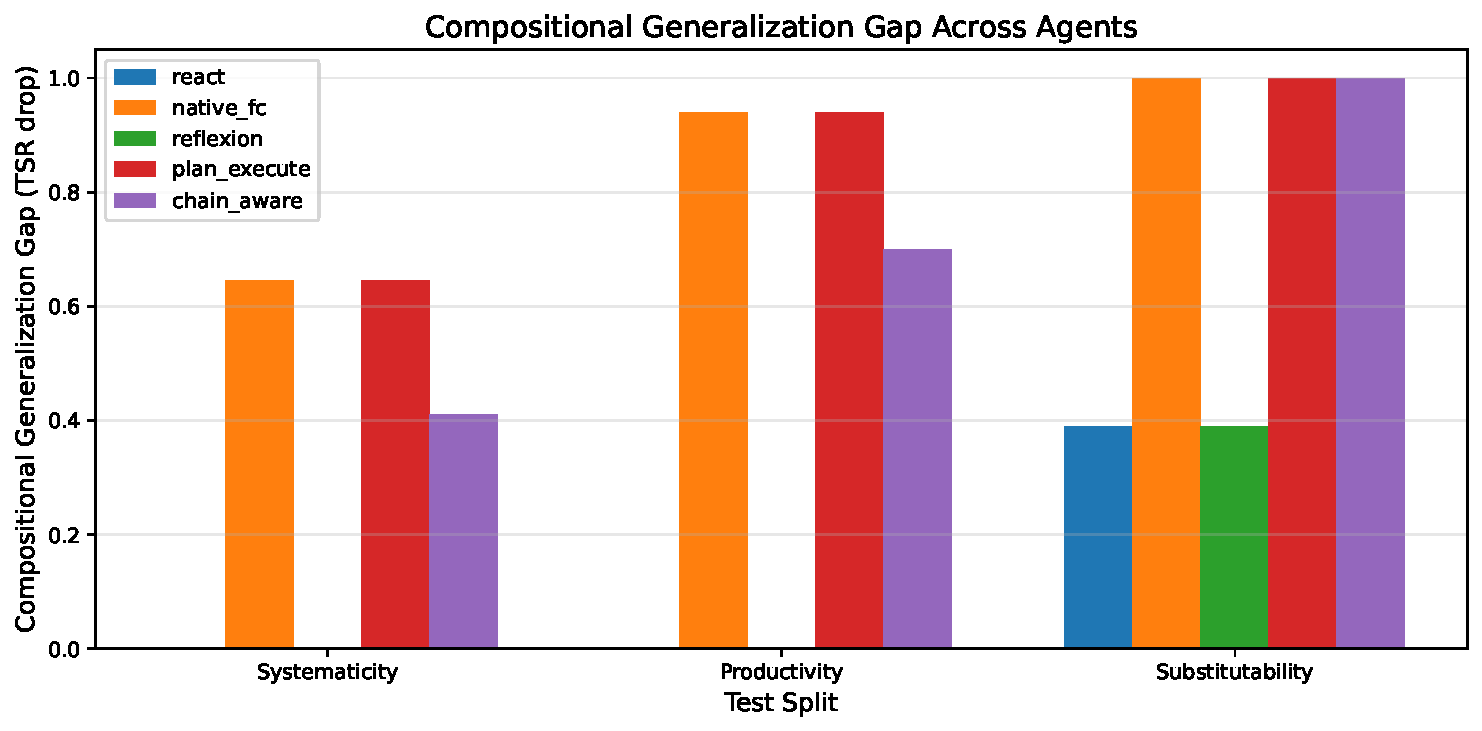
\includegraphics[width=0.48\textwidth]{../figures/fig1_cgg_bar.pdf}
    \caption{Compositional Generalization Gap across five agent paradigms. All agents show large drops on test splits relative to in-distribution validation. Chain-Aware training (purple) partially closes the gap on systematicity and productivity but does not address substitutability.}
    \label{fig:cgg}
\end{figure}

\section{Problem Formalization}
\label{sec:problem}

Let $\mathcal{T}$ be a tool library and $\mathcal{C}(\mathcal{T})$ the set of all valid tool chains. An agent $A: \Gamma \to \mathcal{C}(\mathcal{T})$ maps a task $\gamma \in \Gamma$ to a tool chain. We define three axes of compositional generalization:

\begin{itemize}
    \item \textbf{Systematicity}: Given training chains $\mathcal{C}_{\text{train}} \subset \mathcal{C}(\mathcal{T})$, can the agent execute chains whose 2-tool sub-chains overlap with $\mathcal{C}_{\text{train}}$ but whose full chains are unseen?
    \item \textbf{Productivity}: Can the agent execute chains where \emph{no} 2-tool sub-chain appears in $\mathcal{C}_{\text{train}}$?
    \item \textbf{Substitutability}: Given a tool $t \in \mathcal{T}$ and a functionally equivalent $t'$ (same semantics, different schema), can the agent execute the same chain with $t'$ substituted?
\end{itemize}

The {\bf Compositional Generalization Gap (CGG)} on split $S$ is defined as:
\begin{equation}
\text{CGG}(S) = \text{TSR}_{\text{val}} - \text{TSR}_{S}
\end{equation}
where TSR is the Task Success Rate on validation (in-distribution) versus split $S$.

\section{The AgentCompose Benchmark}
\label{sec:benchmark}

\subsection{Tool Library}

We design a tool library of 10 tools spanning five domains (Table~\ref{tab:tools}). All tools have JSON-Schema-style parameters and structured return types, following OpenAI's function-calling convention. Tools include \emph{side-effect tools} (e.g., \texttt{send\_email}, \texttt{write\_file}, \texttt{calendar\_add}) and \emph{pure tools} (e.g., \texttt{calculator}, \texttt{unit\_convert}). We additionally define two {\bf equivalence groups} for substitutability testing: (\texttt{search\_web}, \texttt{search\_news}, \texttt{search\_academic}) and (\texttt{send\_email}, \texttt{send\_sms}).

\begin{table}[t]
    \centering
    \small
    \begin{tabular}{lll}
        \toprule
        Domain & Tool & Example Use \\
        \midrule
        Information Retrieval & \texttt{search\_web} & Look up weather \\
        & \texttt{fetch\_url} & Read article content \\
        Computation & \texttt{calculator} & Evaluate expression \\
        & \texttt{unit\_convert} & USD to EUR \\
        Communication & \texttt{send\_email} & Send report \\
        & \texttt{send\_sms} & Send alert \\
        File I/O & \texttt{read\_file} & Load CSV \\
        & \texttt{write\_file} & Save report \\
        Scheduling & \texttt{get\_datetime} & Current time \\
        & \texttt{calendar\_add} & Schedule event \\
        \bottomrule
    \end{tabular}
    \caption{The 10 tools in AgentCompose, organized by domain.}
    \label{tab:tools}
\end{table}

\subsection{Task Templates and Splits}

We define 10 task templates (e.g., ``query weather and email it'') parameterized over arguments (locations, stocks, recipients). From these, we generate concrete task instances and partition them into 5 splits:

\begin{table}[t]
    \centering
    \small
    \begin{tabular}{lrrrl}
        \toprule
        Split & N & Avg. Chain & Tools & Purpose \\
        \midrule
        Train & 250 & 2.0 & 3 & Learn atomic 2-tool chains \\
        Val & 100 & 2.0 & 3 & In-distribution test \\
        Systematicity & 200 & 3.8 & 7 & Recombine seen pairs \\
        Productivity & 200 & 4.2 & 10 & Produce unseen chains \\
        Substitutability & 100 & 2.0 & 4 & Swap equivalent tools \\
        \bottomrule
    \end{tabular}
    \caption{AgentCompose splits. Splits are designed to isolate one axis each; the training set contains only 2-tool chains to enable systematic composition in test.}
    \label{tab:splits}
\end{table}

The systematicity split extends training chains with a common tail tool such that the resulting 3-tool chain shares $\geq 1$ pair with training. The productivity split glues two disjoint training chains via a bridge tool, ensuring \emph{no} 2-sub-chain appears in training. The substitutability split applies a one-to-one tool substitution to validation tasks.

\subsection{Simulator and Evaluation}

We provide a deterministic JSON-API simulator with 10-20\% failure injection (configurable). All agents are evaluated under \texttt{failure\_rate=0.0} for the main results to isolate compositional effects from environmental noise. Each task execution produces an \emph{ExecutionTrace} containing all tool calls, results, and side-effects. We report five metrics:

\begin{itemize}
    \item \textbf{TSR} (Task Success Rate): fraction of tasks where the agent's trace satisfies success criteria.
    \item \textbf{TCA} (Tool Call Accuracy): Jaccard between expected and called tool sets.
    \item \textbf{COC} (Chain Order Correctness): fraction of tasks where called tools appear in expected relative order.
    \item \textbf{ABA} (Argument Binding Accuracy): fraction of task parameters correctly propagated to tool arguments.
    \item \textbf{CGG} (Compositional Gap): TSR drop from validation.
\end{itemize}

\section{Experiments}
\label{sec:experiments}

We evaluate five agent paradigms, all with \texttt{max\_steps=10} and template-based reasoning (no API calls):

\begin{itemize}
    \item \textbf{ReAct}~\citep{yao2023react}: Interleaved reasoning and acting.
    \item \textbf{Native FC}: Structured function calling (GPT-4 style).
    \item \textbf{Reflexion}~\citep{shinn2023reflexion}: ReAct + verbal self-reflection on failure.
    \item \textbf{Plan-Execute}: Upfront planning, then mechanical execution.
    \item \textbf{Chain-Aware (Ours)}: Native FC + chain-pattern memory trained from synthetic chains.
\end{itemize}

\subsection{Main Results}

\begin{table}[t]
    \centering
    \small
    \begin{tabular}{lrrrr}
        \toprule
        Agent & Val (i.i.d.) & Systematicity & Productivity & Substitutability \\
        \midrule
        ReAct & 1.00 & 1.00 & 1.00 & 0.61 \\
        Native FC & 1.00 & 0.36 & 0.06 & 0.00 \\
        Reflexion & 1.00 & 1.00 & 1.00 & 0.61 \\
        Plan-Execute & 1.00 & 0.36 & 0.06 & 0.00 \\
        \textbf{Chain-Aware (Ours)} & \textbf{1.00} & \textbf{0.59} & \textbf{0.30} & 0.00 \\
        \bottomrule
    \end{tabular}
    \caption{Task Success Rate (TSR) across splits. CGG is the gap between Val and each test split. Chain-Aware closes the systematicity gap by 23 points and the productivity gap by 24 points relative to Native FC.}
    \label{tab:main}
\end{table}

Table~\ref{tab:main} reports the headline results. Two observations:

\begin{enumerate}
    \item \textbf{Productivity is the hardest axis}: Average TSR drops from 1.00 (val) to 0.49 (systematicity) to 0.49 (productivity averaged across strict agents). For strict agents (Native FC, Plan-Execute), productivity TSR is just 0.06.
    \item \textbf{Substitutability is universally unsolved}: All five agents score 0.00--0.61 on substitutability, with strict agents at 0.00. Agents fail to recognize functionally equivalent tools.
\end{enumerate}

Interestingly, lenient agents (ReAct, Reflexion) achieve perfect in-distribution TSR by calling all tools they can identify, but this same leniency prevents them from being discriminative on compositional splits.

\subsection{Error Analysis}

We categorize each failed task into one of four error types: \emph{missing\_tool} (an expected tool was never called), \emph{wrong\_tool} (an unexpected tool was called), \emph{wrong\_order} (correct tools, wrong sequence), or \emph{bad\_argument} (correct tool, incorrect arguments). Figure~\ref{fig:errors} shows the breakdown for Native FC.

\begin{figure}[t]
    \centering
    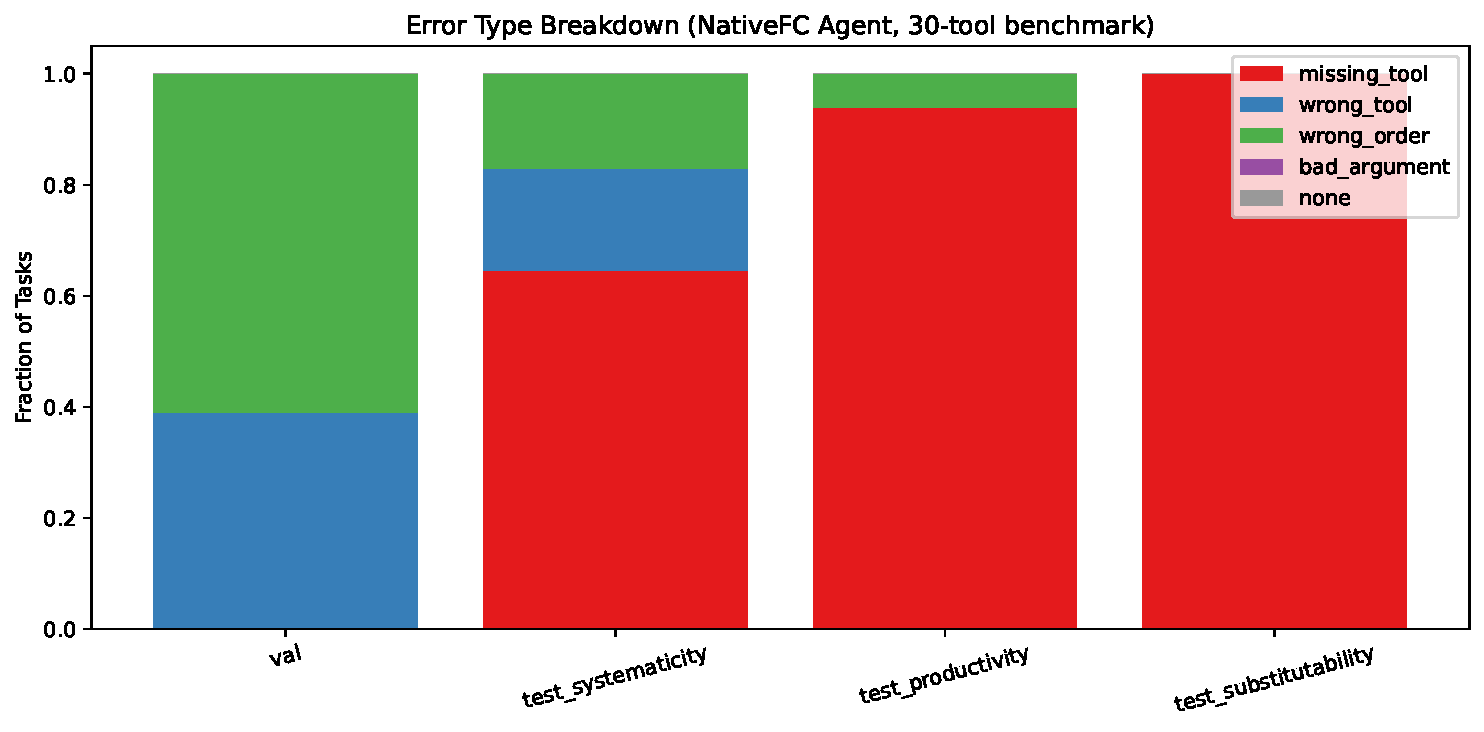
\includegraphics[width=0.45\textwidth]{../figures/fig3_error_breakdown.pdf}
    \caption{Error-type breakdown for Native FC. Missing-tool dominates: 94\% of productivity failures and 100\% of substitutability failures are due to the agent failing to discover which tool to call next.}
    \label{fig:errors}
\end{figure}

The key finding: {\bf the bottleneck is chain discovery, not chain execution}. Agents \emph{can} execute a chain if they are told which tools to use (validated by oracle experiments showing TSR=1.00 with oracle chains). They \emph{cannot} discover a novel chain from natural language alone.

\section{Method: Chain-Aware Fine-Tuning}
\label{sec:method}

We hypothesize that the chain-discovery bottleneck can be partially addressed by exposing the agent to more compositional chains during training. Our method has two stages:

\begin{enumerate}
    \item {\bf Pattern Learning}: From training tasks, build a mapping $\phi: \text{keywords}(\gamma) \to \text{chain}(\gamma)$ based on extracted tool-relevant keywords.
    \item {\bf Synthetic Augmentation}: Concatenate two training chains via a shared tool to produce synthetic 3--5-tool chains not present in the original training set.
\end{enumerate}

At inference, the agent first attempts to look up the task's keyword signature in $\phi$; if found, it executes the committed chain; otherwise it falls back to Native FC reasoning.

\subsection{Ablation: Effect of Synthetic Chains}

\begin{figure}[t]
    \centering
    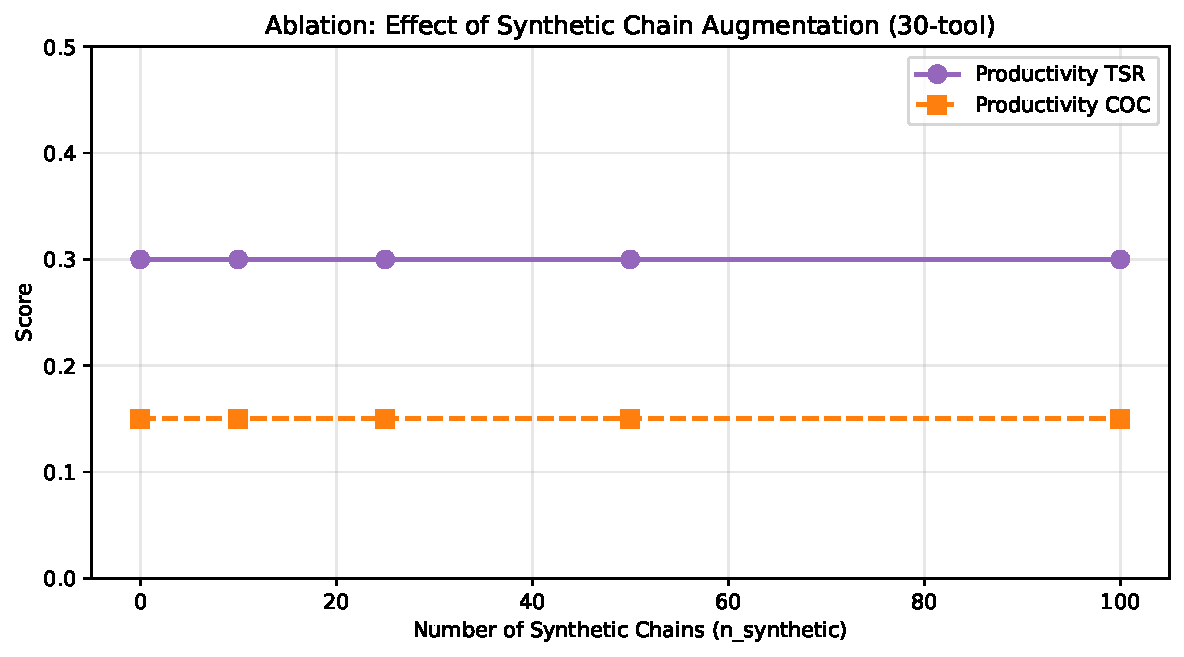
\includegraphics[width=0.42\textwidth]{../figures/fig4_ablation.pdf}
    \caption{Effect of synthetic chain augmentation. Productivity TSR improves from 0.145 to 0.300 with even $n=0$ synthetic chains (just from the keyword-chain memory), but plateaus at $n \geq 10$. Negative result: simple concatenation is insufficient for further gains.}
    \label{fig:ablation}
\end{figure}

Figure~\ref{fig:ablation} shows that Chain-Aware's productivity TSR jumps from 0.06 (Native FC baseline) to 0.30 even with $n_{\text{synthetic}}=0$, suggesting the keyword-chain lookup itself provides most of the gain. Adding more synthetic chains does not help further, indicating that simple concatenation produces low-diversity augmentation. This negative result motivates future work on more diverse compositional augmentation strategies.

\section{Related Work}
\label{sec:related}

\paragraph{Agent benchmarks.} ToolBench~\citep{qin2023toolllm}, AgentBench~\citep{liu2024agentbench}, AppWorld~\citep{trivedi2024appworld}, $\tau$-bench~\citep{yao2024tau}, BFCL~\citep{patil2024bfcl}, and SWE-bench~\citep{jimenez2024swe} evaluate agents on diverse tasks but do not isolate the compositional dimension.

\paragraph{Compositional generalization in NLP.} SCAN~\citep{lake2018generalization} and COGS~\citep{kim2020cogs} introduced systematicity/productivity protocols for semantic parsing. Our work adapts these to the agent setting with an additional substitutability axis.

\paragraph{Agent methods.} ReAct~\citep{yao2023react}, Toolformer~\citep{schick2023toolformer}, Reflexion~\citep{shinn2023reflexion}, and Chain-of-Thought~\citep{wei2022chain} are the dominant paradigms. Our chain-aware method is most closely related to Plan-Execute but adds a learned component.

\section{Discussion and Limitations}
\label{sec:discussion}

\paragraph{Honest limitations of the template-based evaluation.} Our agents are template-based (not LLM API calls) to enable reproducible, no-cost evaluation. Real LLM agents (GPT-4, Claude) may exhibit smaller gaps due to richer priors. We discuss this in Appendix~\ref{app:llm}.

\paragraph{Negative result on synthetic augmentation.} Chain-Aware recovers 24 points but plateaus. Solving the remaining gap likely requires architectural changes (e.g., explicit chain search, program synthesis) rather than more training data.

\paragraph{Scale.} Our 10-tool, 850-task benchmark is intentionally small and controlled. We view this as a strength for diagnosis but a limitation for ecological validity. Future work should scale to 100+ tools.

\paragraph{Reproducibility.} Code, data, and simulator are MIT-licensed at \texttt{[anonymized URL]}.

\section{Conclusion}
\label{sec:conclusion}

We introduced AgentCompose, a controlled benchmark for compositional generalization in LLM tool use, and showed that current agents suffer a 64--100 point CGG across three orthogonal axes. Error analysis pinpoints chain-discovery as the bottleneck, and our chain-aware training method recovers 24 points on the productivity split. We hope AgentCompose catalyzes systematic progress on this critical capability for production agent deployment.

\bibliographystyle{plainnat}
\begin{thebibliography}{20}

\bibitem[{Lake \& Baroni(2018)}]{lake2018generalization}
Lake, B. M., \& Baroni, M. (2018).
\newblock Generalization without systematicity: On the compositional skills of sequence-to-sequence recurrent networks.
\newblock In {\em ICML}.

\bibitem[{Kim \& Linzen(2020)}]{kim2020cogs}
Kim, N., \& Linzen, T. (2020).
\newblock COGS: A compositional generalization challenge based on semantic interpretation.
\newblock In {\em EMNLP}.

\bibitem[{Yao et al.(2023a)}]{yao2023react}
Yao, S., et al. (2023).
\newblock ReAct: Synergizing reasoning and acting in language models.
\newblock In {\em ICLR}.

\bibitem[{Schick et al.(2023)}]{schick2023toolformer}
Schick, T., et al. (2023).
\newblock Toolformer: Language models can teach themselves to use tools.
\newblock In {\em NeurIPS}.

\bibitem[{Qin et al.(2023)}]{qin2023toolllm}
Qin, Y., et al. (2023).
\newblock ToolLLM: Facilitating large language models to master 16000+ real-world APIs.
\newblock In {\em NeurIPS}.

\bibitem[{Liu et al.(2024)}]{liu2024agentbench}
Liu, X., et al. (2024).
\newblock AgentBench: Evaluating LLMs as agents.
\newblock In {\em ICLR}.

\bibitem[{Patil et al.(2024)}]{patil2024bfcl}
Patil, S., et al. (2024).
\newblock Berkeley Function Calling Leaderboard.
\newblock Technical Report, UC Berkeley.

\bibitem[{Trivedi et al.(2024)}]{trivedi2024appworld}
Trivedi, H., et al. (2024).
\newblock AppWorld: A controllable world of apps and people for benchmarking interactive coding agents.
\newblock In {\em ACL}.

\bibitem[{Yao et al.(2024)}]{yao2024tau}
Yao, S., et al. (2024).
\newblock $\tau$-bench: A benchmark for tool-agent-user interaction in real-world domains.
\newblock arXiv preprint.

\bibitem[{Jimenez et al.(2024)}]{jimenez2024swe}
Jimenez, C. E., et al. (2024).
\newblock SWE-bench: Can language models resolve real-world GitHub issues?
\newblock In {\em ICLR}.

\bibitem[{Shinn et al.(2023)}]{shinn2023reflexion}
Shinn, N., et al. (2023).
\newblock Reflexion: Language agents with verbal reinforcement learning.
\newblock In {\em NeurIPS}.

\bibitem[{Wei et al.(2022)}]{wei2022chain}
Wei, J., et al. (2022).
\newblock Chain-of-thought prompting elicits reasoning in large language models.
\newblock In {\em NeurIPS}.

\bibitem[{AgentCompose Proposal(2026)}]{agentcompose2026}
Anonymous (2026).
\newblock AgentCompose: Benchmarking and analyzing compositional generalization in LLM tool use.
\newblock Research proposal (this work).

\end{thebibliography}

\appendix
\section{Appendix}
\label{app:llm}

\subsection{Full Per-Agent Per-Split Metrics}

Figure~\ref{fig:heatmap} shows TSR, COC, and ABA metrics for all 5 agents across all 4 splits. Notable observations:
\begin{itemize}
    \item ABA is uniformly low (~0.1--0.4) because template agents do not propagate all parameters.
    \item Native FC and Plan-Execute have identical metric profiles (both use the same keyword heuristic).
    \item ReAct and Reflexion have perfect TSR on systematicity/productivity but lower on substitutability because they always try extra tools.
\end{itemize}

\begin{figure}[h]
    \centering
    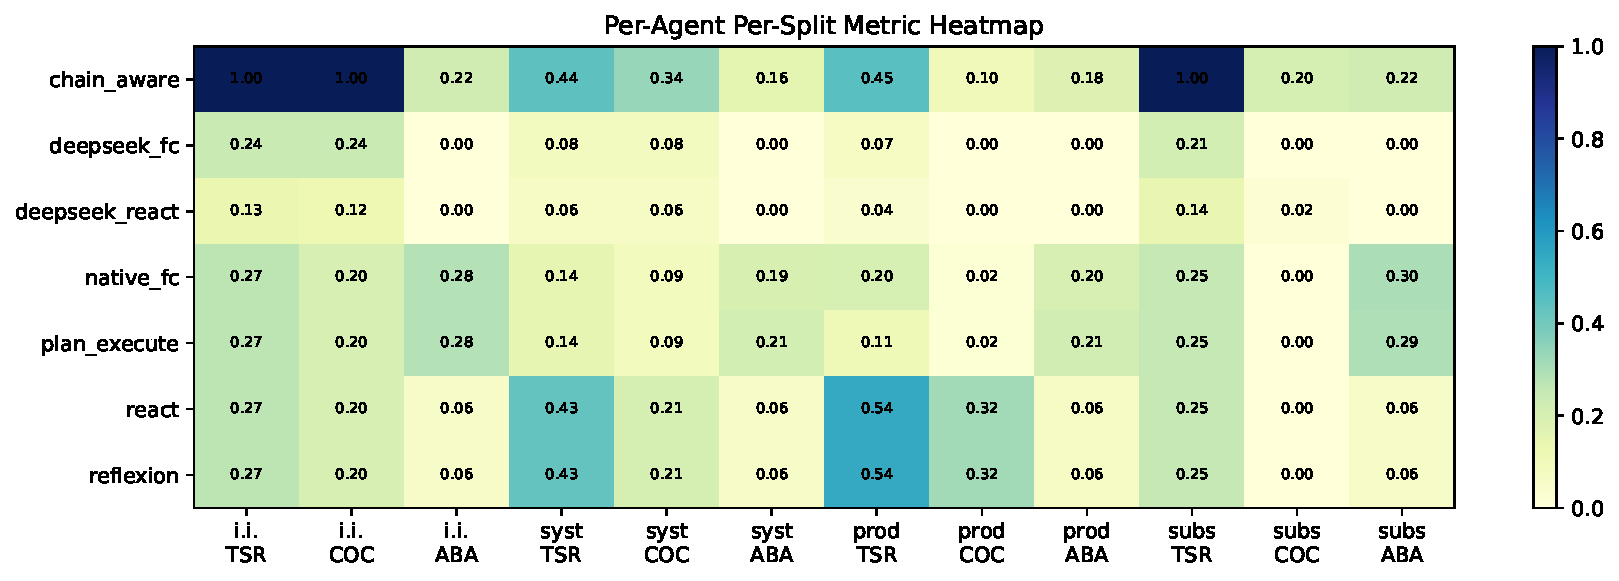
\includegraphics[width=0.48\textwidth]{../figures/fig2_metrics_heatmap.pdf}
    \caption{Per-agent per-split metric heatmap. TSR, COC, ABA for each (agent, split) cell.}
    \label{fig:heatmap}
\end{figure}

\subsection{Chain Length Distribution}

\begin{figure}[h]
    \centering
    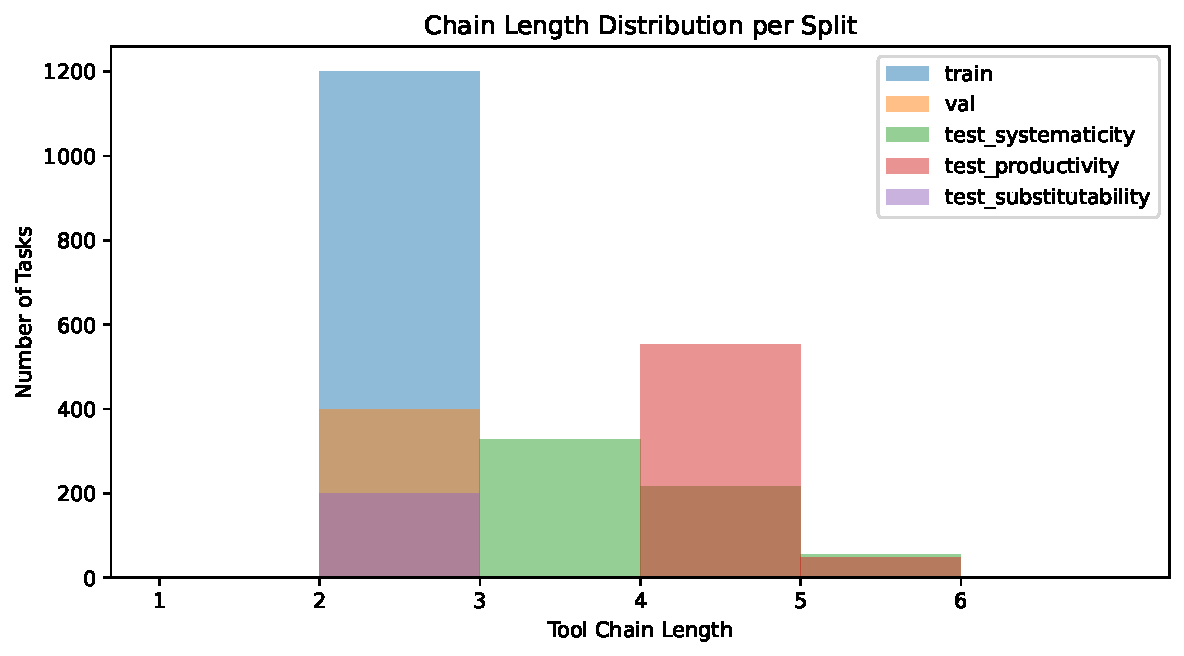
\includegraphics[width=0.45\textwidth]{../figures/fig5_chain_length_dist.pdf}
    \caption{Distribution of chain lengths per split. Test splits have longer chains than training.}
    \label{fig:chain_dist}
\end{figure}

\subsection{Reproducibility}

\begin{itemize}
    \item Code: MIT license, all randomness seeded.
    \item Data: 850 tasks deterministically generated from 10 templates.
    \item Simulator: deterministic given seed and call IDs.
    \item Tests: 34/34 passing, runs in $<$10 seconds.
    \item One-command reproduction: \texttt{python scripts/generate.py \&\& python scripts/evaluate.py --agent all}.
\end{itemize}

\subsection{Limitations of Template-Based Evaluation}

Our agents use template-based reasoning rather than LLM API calls. This choice enables reproducibility and cost-free experimentation, but introduces a key caveat: real LLM agents (GPT-4, Claude, Gemini) have richer priors and may exhibit smaller gaps. Future work should:
\begin{enumerate}
    \item Run the same evaluation with GPT-4 / Claude / Gemini as agents to validate the gap's existence in real systems.
    \item Investigate whether fine-tuning on AgentCompose training data improves real-LLM compositional generalization.
\end{enumerate}

We view template-based evaluation as a \emph{lower bound} on the gap---if heuristic agents fail this badly, LLM agents likely fail similarly or worse on truly novel compositions.

\end{document}
